\section{Benutzungsoberfläche}


\subsection{Startfenster}

\begin{figure}[hp] 
  \centering
     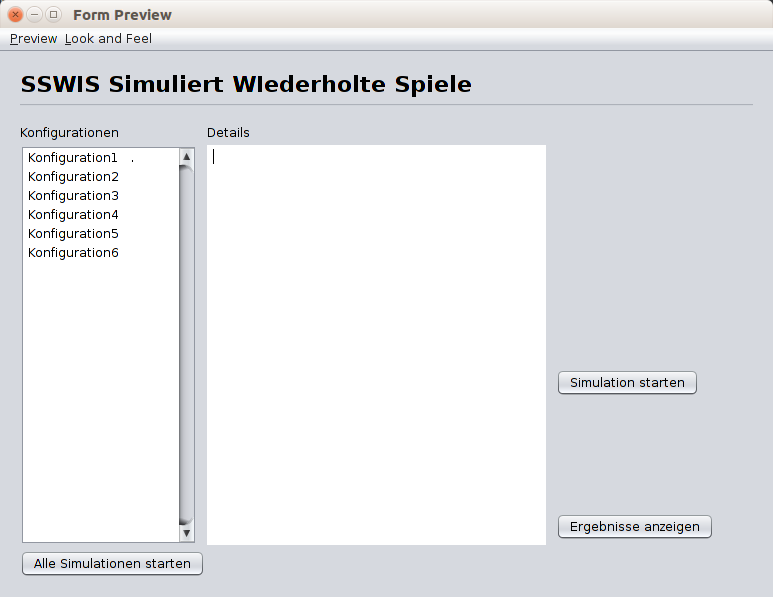
\includegraphics[width=1.1\textwidth]{GUI_Entwurf/Startfenster.png}
  \caption{Hauptfenster}
  \label{fig:Bild1}
\end{figure}

\begin{description}


\item[1. Menü Stufenspiele] Enthält den Menüpunkt 'Stufenspiele verwalten'. Dieser führt zur Stufenspiel Verwaltung.

\item[2. Menü Strategien] Enthält den Menüpunkt 'Kombinierte Strategien verwalten'. Dieser führt zu dem Kombinierte Strategien Verwaltung.

\item[3. Menü Initialisierungen] Enthält Menüpunkt 'Initialisierungen bearbeiten' und 'Neue Initialisierung'. 'Initialisierungen bearbeiten' öffnet ein OpenFileDialog in dem Initialisierungen gelöscht, umbenannt und in das Initialisierungsfenster geöffnet und bearbeitet werden können. 'Neue Initialisierung' öffnet das Initialisierungs-Fenster.

\item[4. Menü Konfigurationen] Enthält Menüpunkt 'Neue Konfiguration'. Dieser öffnet das Konfigurations-Fenster.

\item[5. Menü Ergebnisse] Enthält Menüpunkt 'Ergebnisse vergleichen'. Dieser öffnet das Vergleichfenster.

\item[6. Liste der Konfigurationen] Diese zeigt die Liste der erstellten Konfigurationen an. Werden neue Konfigurationen erstellt, werden die vorigen Konfigurationen durch die Neuen in der Liste ersetzt.

\item[7. Details] Ist eine Konfiguration in der Liste ausgewählt, werden hier die Parameter der Konfiguration angezeigt.

\item[8. Simulation starten] Ist eine Konfiguration in der Liste ausgewählt, ist dieser Button aktiviert. Nach dem Betätigen wird in einem Pop-Up-Fenster die Anzahl der Wiederholungen abgefragt. Danach wird die Simulation gestartet.

\item[9. Ergebnisse anzeigen] Wurde eine Simulation mit der in der Liste ausgewählten Konfiguration durchgeführt, ist dieser Button aktiviert. Er öffnet das Ergebnisfenster mit den Ergebnissen, der letzten Durchführung.

\item[10. Alle Simulationen starten] Nach dem Betätigen wird in einem PopUpFenster die Anzahl der Wiederholungen abgefragt. Danach werrden die Simulationen für alle Konfigurationen in der Liste gestartet.

\end{description}

\pagebreak

\subsection{Stufenspiele Verwaltung}

\begin{figure}[hp] 
  \centering
     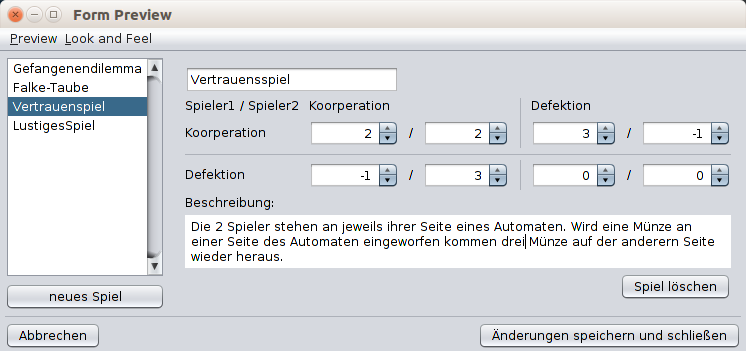
\includegraphics[width=1.1\textwidth]{GUI_Entwurf/SpieleMenue.png}
  \caption{Stufenspiel Verwaltung}
  \label{fig:Bild1}
\end{figure}

\begin{description}

\item[1. Liste] Zeigt alle zuvor gespeicherten und voreingestellten Stufenspiele. Wird ein Spiel ausgewählt erscheinen alle Parameter in den Feldern zwei bis vier rechts neben der Liste.

\item[2. Name] Der Name des Stufenspiels lässt sich bearbeiten.

\item[3. Auszahlungen] Alle acht Felder für die Auszahlung, lassen sich bearbeiten.

\item[4. Beschreibung] Es lässt sich eine Beschreibung für das Spiel angeben.

\item[5. neues Spiel] Fügt ein neues Stufenspiel in die Liste an. 

\item[6. Spiel löschen] Das in der Liste ausgewählte Spiel wird gelöscht.

\item[7. Abbrechen] Alle zuvor vorgenommen Änderungen inklusive das Erstellen neuer Spiele werden verworfen und die Spiele Verwaltung schließt sich.

\item[8. Änderungen speichern und schließen] Alle zuvor vorgenommen Änderungen werden gespeichert und die Spiele Verwaltung schließt sich.

\end{description}

\pagebreak

\subsection{Kombinierte Strategien Verwaltung}


\begin{figure}[hp]
  \centering
     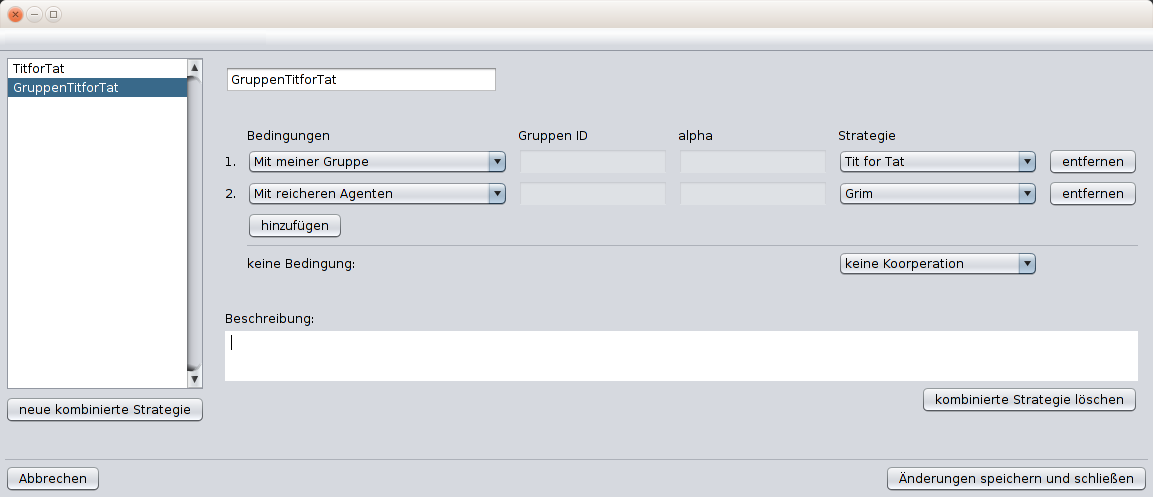
\includegraphics[width=1.15\textwidth]{GUI_Entwurf/StrategienMenue.png}
  \caption{Kombinierte Strategien Verwaltung}
  \label{fig:Bild1}
\end{figure}

\begin{description}

\item[1. Liste] Zeigt alle zuvor gespeicherten kombinierten Strategien. Wird eine kombinierte Strategie ausgewählt, erscheinen alle Parameter in den Feldern zwei bis elf rechts neben der Liste.

\item[2. Name] Der Name der kombinierten Strategie kann geändert werden.

\item[3. Nummerierung] Gibt die Reihenfolge an nach denen Bedingungen geprüft werden.

\item[4. Bedingung] Bedingung, mit der die rechten Strategie gewählt wird.

\item[5. Gruppen ID] Ist aktiviert, wenn Bedingung 'mit Gruppe \textit{Gruppen ID}' ausgewählt ist. Hier kann die entsprechende ID der Gruppe eingegeben werden.

\item[6. alpha] Ist aktiviert wenn Bedingung 'mit Wahrscheinlichkeit \textit{Gruppen alpha}' ausgewählt ist. Hier kann die entsprechende Wahrscheinlichkeit eingegeben werden.

\item[7. Strategie] Die Strategie, die eintreten soll, wenn die Bedingung links daneben erfüllt ist.

\item[8. entfernen] Entfernt diese Zeile mit den entsprechenden Feldern drei bis sieben. Die Nummerierung wird entsprechend angepasst.

\item[9. hinzufügen] Fügt eine Zeile mit den entsprechenden Feldern drei bis sieben an. Die Nummerierung wird entsprechend fortgesetzt.

\item[10. keine Bedingung] Strategie die ausgeführt, wenn keine der ausgewählten Bedingungen erfüllt ist.

\item[11. Beschreibung] Kombinierten Strategien kann eine Beschreibung hinzugefügt werden.

\item[12. neue kombinierte Strategie] Fügt eine neue kombinierte Strategie in die Liste an. 

\item[13. kombinierte Strategie löschen] Die in der Liste ausgewählte kombinierte Strategie wird gelöscht.

\item[14. Abbrechen] Alle zuvor vorgenommen Änderungen inklusive das Erstellen neuer kombinierter Strategien werden verworfen und die Kombinierte Strategien Verwaltung schließt sich. 

\item[15. Änderungen speichern und schließen] Alle zuvor vorgenommen Änderungen werden gespeichert und die Kombinierte Strategien Verwaltung schließt sich.

\end{description}

\pagebreak

\subsection{Initialisierung erstellen}

\begin{figure}[!hp] 
  \centering
     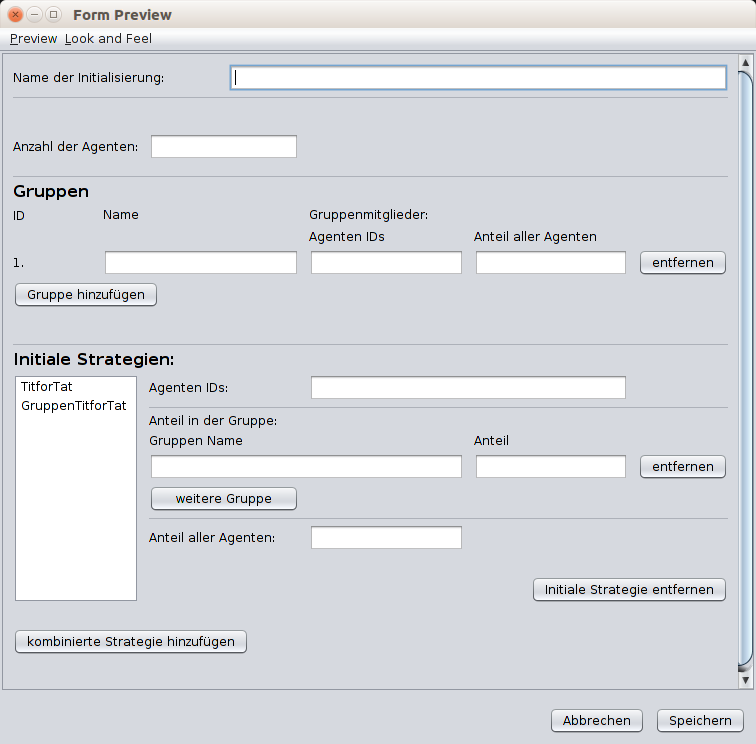
\includegraphics[width=1.1\textwidth]{GUI_Entwurf/NeueInitialisierung.png}
  \caption{Initialisierung}
  \label{fig:Bild1}
\end{figure}


\begin{description}


\item[1. Name] Name der Initialisierung.

\item[2. Anzahl der Agenten] Anzahl der Agenten soll hier angegeben werden. Es können auch variable Werte der Form \textit{Startwert - Endwert - Schrittweite} eingegeben werden.

\item[3. Gruppen - ID] Die Gruppen ID wird automatisch vergeben.

\item[4. Gruppen - Name] Der Gruppen Name soll hier angegeben werden.

\item[5. Gruppen - AgentenIDs] Hier können einzelne IDs und ID Intervalle von Agenten dieser Gruppe angegeben werden. 

\item[6. Gruppen - Anteil aller Agenten] Hier kann ein prozentualer Anteil aller Agenten in dieser Gruppe angegeben werden. Es können auch variable Werte der Form \textit{Startwert - Endwert - Schrittweite} eingegeben werden.

\item[7. Gruppen - entfernen] Entfernt die Zeile mit den Feldern drei bis sechs. Die IDs der Gruppen werden entsprechend angepasst. 

\item[8. Gruppen - Gruppe hinzufügen] Fügt eine neue Zeile mit den Feldern drei bis sechs an. Die ID wird entsprechend vergeben.

\item[9. Initiale Strategien - Liste] Enthält alle initialen kombinierten Strategien. Die Parameter für den Anteil der in der Liste ausgewählte initiale Strategie werden rechts neben der Liste angezeigt. 

\item[10. Initiale Strategien - Agenten IDs] Hier können einzelne IDs und ID Intervalle von Agenten mit dieser Strategie angegeben werden. 

\item[11. Initiale Strategien - Gruppen Name] Hier kann eine Gruppe mit ihrem Namen angegeben werden, zu der der Anteil der Agenten mit der gewählten Strategie angegeben werden soll.

\item[12. Initiale Strategien - Anteil] Anteil der Agenten in der Gruppe mit der gewählten Strategie soll hier angegeben werden. Es können auch variable Werte der Form \textit{Startwert - Endwert - Schrittweite} eingegeben werden.

\item[13. Initiale Strategien - entfernen] Entfernt die Zeile mit den Feldern elf und zwölf.

\item[14. Initiale Strategien - weitere Gruppe] Fügt eine Zeile mit den Feldern elf und zwölf an.

\item[15. Initiale Strategien - Anteil der Agenten] Hier kann der Anteil aller Agenten mit dieser Initialen Strategie angegeben werden. Es können auch variable Werte der Form \textit{Startwert - Endwert - Schrittweite} eingegeben werden.

\item[17. Initiale Strategien - Initiale Strategie entfernen] Entfernt die ausgewählte initiale Strategie aus der Liste. 

\item[17. Initiale Strategien - kombinierte Strategie hinzufügen] 

\item[18. Abbrechen] Alle Änderungen werden verworfen und das Fenster wird geschlossen.

\item[19. Speichern] Alle Änderungen werden gespeichert und das Fenster wird geschlossen.

\end{description}




\subsection{Konfigurationen erstellen}

\begin{figure}[!hp] 
  \centering
     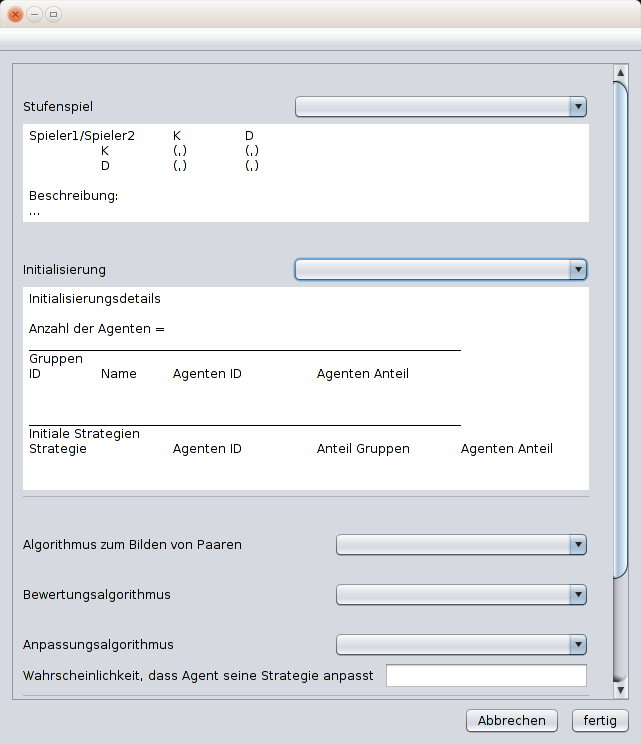
\includegraphics[width=1.0\textwidth]{GUI_Entwurf/NeueKonfiguration1.png}
  \caption{Konfiguration}
  \label{fig:Bild2}
\end{figure}



\begin{description}

\item[1. Stufenspiel] Hier kann eines von den gespeicherten und voreingestellten Stufenspielen ausgewählt werden. Im Textfeld darunter werden Informationen zum ausgewählten Stufenspiel angegeben.

\item[2. Initialisierung] Hier kann eine zuvor gespeicherte Initialisierung ausgewählt werden. Im Textfeld darunter werden Informationen zur ausgewählten Initialisierung angegeben.

\item[3. Algorithmus zum Bilden von Paaren] Hier soll ein Algorithmus zum Bilden von Paaren gewählt werden. 

\item[4. Bewertungsalgorithmus] Hier soll ein Algorithmus zum Bilden von Paaren gewählt werden.

\item[5. Anpassungsalgorithmus] Hier soll ein Algorithmus zum Bilden von Paaren gewählt werden.

\item[6. Wahrscheinlichkeit für Strategieanpassung] Hier soll die Wahrscheinlichkeit für Strategieanpassung angegeben werden. Es können auch variable Werte der Form \textit{Startwert - Endwert - Schrittweite} eingegeben werden.

\begin{figure}[!h] 
  \centering
     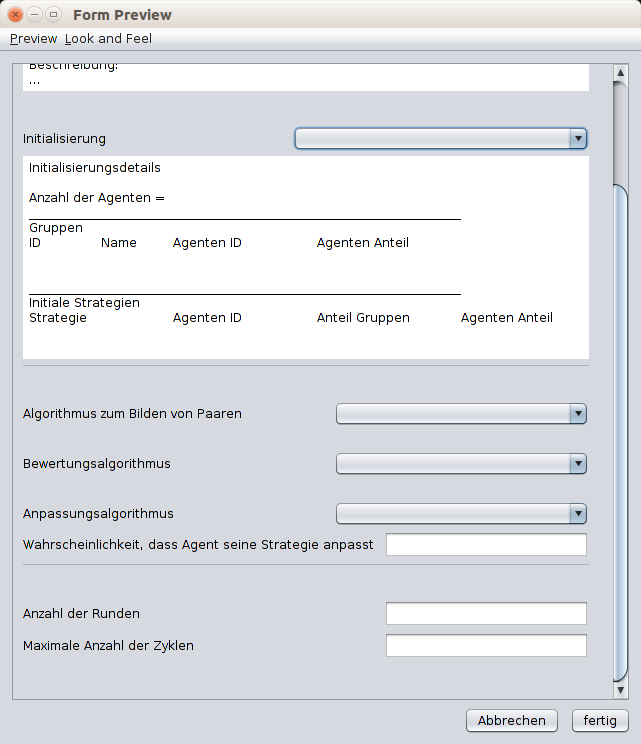
\includegraphics[width=1.0\textwidth]{GUI_Entwurf/NeueKonfiguration2.png}
  \caption{Konfiguration}
  \label{fig:Bild2}
\end{figure}

\item[7. Anzahl der Runden] Hier soll die Anzahl der Runden angegeben werden. Es können auch variable Werte der Form \textit{Startwert - Endwert - Schrittweite} eingegeben werden.

\item[8. Maximale Anzahl der Zyklen] Hier soll die maximale Anzahl der Zyklen angegeben werden. Es können auch variable Werte der Form \textit{Startwert - Endwert - Schrittweite} eingegeben werden.

\item[9. fertig] Das Fenster wird geschlossen und die durch die Parameter bestimmten Konfigurationen werden auf die Startseite geladen.

\item[10. Abbrechen] Alle Eingaben werden verworfen und das Fenster wird geschlossen.


\end{description}

\pagebreak


\subsection{Ergebnisse anzeigen}

\begin{figure}[!hp] 
  \centering
     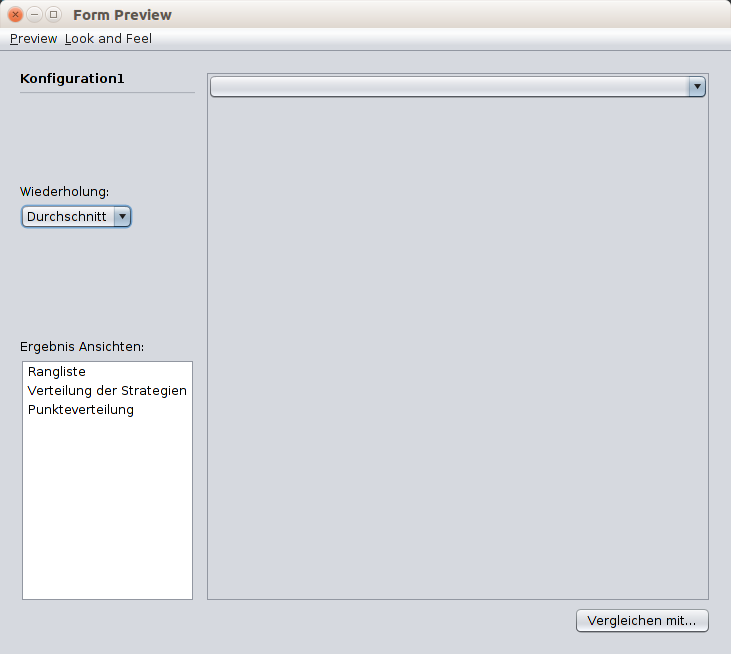
\includegraphics[width=1.1\textwidth]{GUI_Entwurf/Ergebnisfenster(1).png}
  \caption{Ergebnisfenster}
  \label{fig:Bild7}
\end{figure}

\begin{description}

\item[1. Konfiguration] Die Konfiguration, die für die Simulation verwendet wurde.

\item[2. Wiederholung] Es kann zwischen den einzelnen Wiederholungen der Simulation oder dem Durchschnitt gewählt werden, zu denen die Ergebnisse angezeigt werden.

\item[3. Liste Ergebnis Ansichten] Es gibt verschiedene Details, die dem Nutzer graphisch angezeigt werden können. Die entsprechenden Daten und Graphiken werden rechts im Ansicht Panel angezeigt.

\item[4. Ansicht] In diesem Panel werden die Ergebnis-Graphiken angezeigt. Bei Graphiken die verschiedene Optionen bieten, kann zwischen diesen im oberen DropDownMenü gewählt werden.

\item[5. Vergleichen mit...] Öffnet das Vergleichfenster. Die Konfiguration ist in der linken Spalte bereits ausgewählt.

\end{description}

\pagebreak


\subsection{Ergebnisse vergleichen}

\begin{figure}[!hp] 
  \centering
     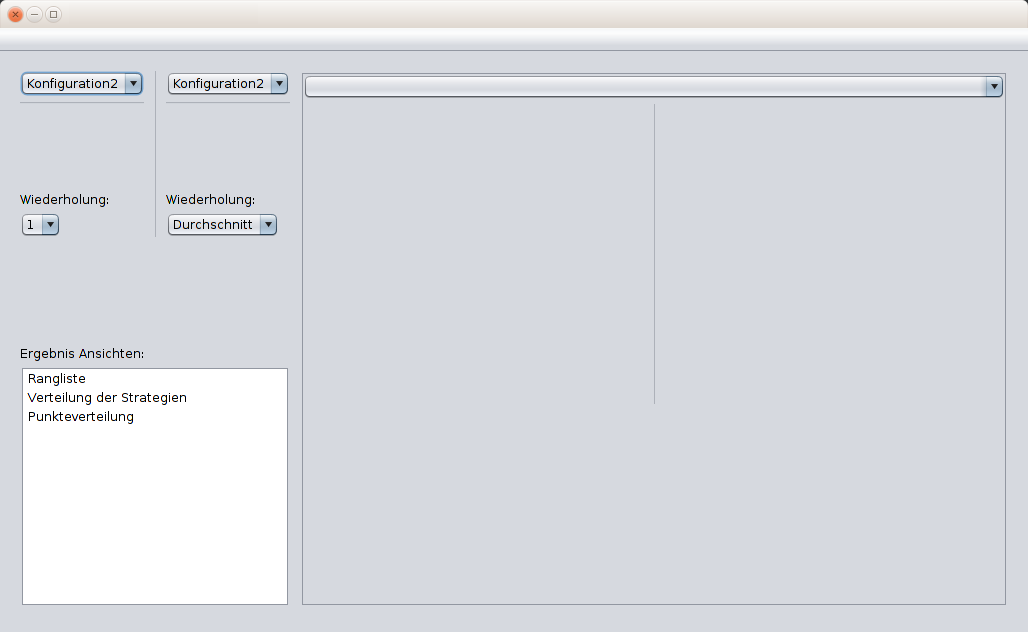
\includegraphics[width=1.15\textwidth]{GUI_Entwurf/Vergleichfenster.png}
  \caption{Vergleichenfenster}
  \label{fig:Bild1}
\end{figure}

\begin{description}

\item[1. Konfiguration] In den zwei Spalten können die Konfigurationen gewählt werden, deren Simulationen verglichen werden sollen.

\item[2. Wiederholung] Ebenso kann zu jeder Konfiguration die Wiederholung oder der Durchschnitt gewählt, um zu bestimmen, welche Ergebnisse miteinander verglichen werden sollen.

\item[3. Liste Ergebnis Ansichten] Es gibt verschiedene Details, die dem Nutzer graphisch angezeigt werden können. Die entsprechenden Daten und Graphiken werden rechts im Ansicht Panel angezeigt.


\item[4. Ansicht] In diesem Panel werden in der jeweiligen Spalte die ausgewählte Ergebnissansicht zu der entsprechenden Konfiguration angezeigt. Unter den Spalten wird die Differenz, der beiden Ergebnisse angegeben. Bei Graphiken, die verschiedene Optionen bieten, kann zwischen diesen im oberen DropDownMenü gewählt werden.

\end{description}



